\documentclass[12pt,a4paper]{report}

\usepackage[utf8x]{inputenc}
\usepackage[left=2cm, right=2cm, top=5cm]{geometry}
\usepackage{enumitem}
\usepackage{fontspec}
\usepackage{tikz}
\usetikzlibrary{graphs, shapes, snakes, graphdrawing}

\begin{document}

\begin{titlepage}
	\centering
	{\scshape\LARGE Universidad Nacional Autónoma de México \par}
	\vspace{1cm}
	{\scshape\Large Computación Distribuida\par}
	\vspace{1.5cm}
	{\huge\bfseries Tarea 5\par}
	\vspace{.5cm}
	{\Large\itshape Edgar Quiroz Castañeda \par}
    \vspace{.5cm}
	{\Large\itshape Jerónimo Almeida Rodríguez \par}
	\vfill
	 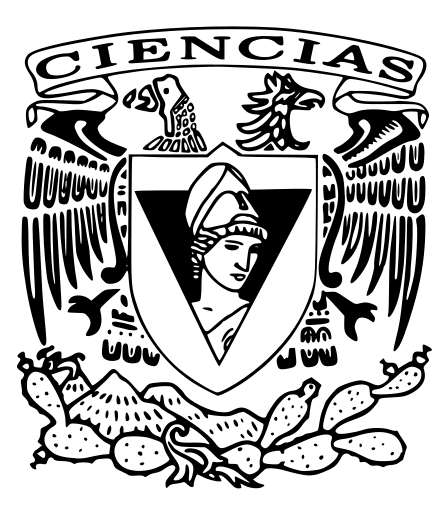
\includegraphics[width=0.5\textwidth]{escudo_f-ciencias.png}
	\vfill

% Bottom of the page
	{\large Jueves 27 de septiembre del 2018 \par}
\end{titlepage}

\pagebreak
\setlength{\voffset}{-0.75in}
\setlength{\headsep}{5pt}

\newcommand{\is}[1]{V_{\{#1, x, r\}}} %Invariante de ciclo para la dem. del algoritmo

\begin{enumerate}
	%Ejercicio 1
	\item {
		Considere la gráfica $G$. Propón retardos y ejecuta el algoritmo PIF con
		$p_1$ como raíz.\\
	}

	%Ejercicio 2
	\item {
		En la Ciudad de México varios puntos de control (nodos) fueron agregados.\\
		Cada uno de estos puntos tiene información de cuantas personas viven
		dentro de cierto diámetro. \\
		Un punto (raíz) de la delegacion Benito Juárez quiere recolectar la
		información de todos los puntos de control. \\
		Escribe un algoritmo para que cada nodo recolecte la información de sus
		hijos para enviarsela al padre sin repetirla.\\
		}

	%Ejercio 3
	\item{
		Demuestre por inducción que en el algoritmo PI, cada nodo $v$ recibe el
		mensaje $M$ por primera vez en a lo más $d(root, v)$.\\
	}
	%Ejercio 4
	\item{
		Se dice que una digráfica $G = (V, E)$ tiene raiz $r$ si $r \in V$ y cada
		vértice $v \in V$ es alcanzable desde $r$, es decir, existe un camino
		dirigido alcanzable desde $r$ (un camino dirigido que empieza en $r$ y
		termina en $v$).\\
		Una digráfica $G$ es un  ́arbol dirigido si tiene raíz y la versión no dirigida
		de $G$ es un árbol. Demuestra el siguiente teorema:\\

		\textbf{Teorema 1}\\
		Sea G una digráfica. Las siguientes condiciones son equivalentes
		\begin{enumerate} [label = \alph*)]
			\item {
				$G$ es un árbol dirigido.\\
			}
			\item {
				$G$ tiene una raíz desde la cual hay un único camino dirigido a
				vértice.\\
			}

			\item{
				$G$ tiene una raíz $r$ para la cual $\delta(r)_{in} = 0$, y para cualquier
				otro vértice $v$, $\delta_{in}(v) = 1$.\\
			}

			\item{
				$G$ tiene una raíz $r$ y el quitar cualquier arista interumpe la
				condición.
			}
			\item{
				La versión no dirigida de $G$ es conexa y $G$ tiene un vértice $r$ para
				el cual $\delta_{in}(t) = 0$ mientras que para cualquier otro vértice
				$v$ $\delta(v)_{in} = 1$.
			}
		\end{enumerate}
	}

\end{enumerate}
\end{document}
